%%==================================================
%% chapter02.tex for BIT Master Thesis
%% modified by liu xiahua
%% version: 0.1
%% last update: May 20th, 2018
%%==================================================

\chapter{电池箱机械设计}
\label{chap:engineering}

在本章,本文将会就上一章所设计的电池箱系统参数,对于该电池箱进行机械结构的设计和校核,混合动力汽车的电池箱结构设计与纯电动汽车的电池箱结构基本类似,但是由于其电池的数量较少,所以混合动力电池箱的结构较为简单,但是设计的时候应该遵守电池箱设计标准。因为车载电池的工作环境较差,电池箱需要承受来自车身的振动 ,加速度,以及电池箱内部产生的热量,在国外,有研究认为,环境温度,压力,机械振动等电池包所在的长期环境条件,会对电池可靠性产生重大影响 \cite{王文伟2016电动汽车电池箱结构随机振动疲劳分析}。也有研究认为,温度也影响锂离子电池包的可靠性和电池的循环寿命 \cite{能量效率和工作温度对锂离子电池剩余寿命的影响}。所以电池箱的结构设计在电动汽车领域占有一定的比重。

\section{现有标准相关信息}

由于目前电动车市场已经逐渐成熟,电池箱结构与安全方面的相关的标准制定已经相当完善,在美国 SAE 协会制定了许多相关的电动车标准,如表 \ref{tab:SAE_standard} 所示,电池箱相关的结构设计标准在电池极耳和母线的连接方式,电池的布置方面进行了详细的叙述,对于电池的热失控的控制等安全性问题也进行了相关的解决方案的规定,对于电池系统的热管理系统进行了方案的提出。

传统的电池箱设计是针对于电池箱模组的安全设计和检查的,本文对于电池箱的模组设计充分考虑到了安全因素,并且在模组范围之外,本文还对于电池箱整体与车体的连接进行了设计校核 \cite{Dubarry2009From}。在电池与车辆的连接部分处承受着来自电池箱的巨大重量,并且由于第一章匹配对应的电池箱的质量较重,故其惯性较大,在车辆产生振动或者加速减速的状态下,电池箱安装框架连接部分会产生较大的应力,故校核框架的连接强度是十分必要的。

\begin{table}
	\centering
	\caption{SAE 对于电池箱机械结构和安全方面的标准} \label{tab:SAE_standard}
	\begin{tabular*}{0.9\textwidth}{@{\extracolsep{\fill}}cp{5cm}p{5cm}}
		\toprule
		\textbf{标准} & \textbf{题目} & \textbf{简介} \\
		\midrule
		SAE J240 & Life test for Automotive Storage batteries & 车载电池寿命测试 \\
        SAE J1766 & Recommended Practice for EV \& Hybrid Vehicle Battery Systems Crash Integrity Testing & 电动汽车电池系统碰撞完整性测试\\
        SAE J1797 & Packaging of Electric Vehicle Battery Modules & 电动汽车电池模组包装\\
        SAE J1798 & Recommended Practice for Performance Rating of Electric Vehicle Battery Modules & 电动汽车电池模组测试和性能评级 \\
        SAE J2185 & Life test for heavy-duty Storage batteries & 重型汽车的寿命测试\\
        SAE J2289 & Electric-Drive Battery Pack System: Functional Guidelines & 电动汽车电池包系统的功能设计方针\\
        SAE J2344 & Technical Guidelines for Electric Vehicle Safety & 电动汽车安全性技术指导\\
        SAE J2380 & Vibration Testing of Electric Vehicle Batteries & 电动汽车的振动测试\\
        SAE J2929 & Electric and Hybrid Vehicle Propulsion Battery System Safety Standard & 电动汽车动力电池的安全标准\\
		\bottomrule
	\end{tabular*}
\end{table}


在第二章节内,本文通过计算设计确定,电池包的总电池单体数量为 88 块,在进行机械设计前,通过对于现有的商用车型上电池箱设计方案的参考,了解到了目前的电池箱设计分为: 单体级别的设计,模块级别的设计,电池包总体设计,首先进行的是电池在单体级别的设计。

\section{电池单体级别设计}
电池单体的尺寸来自天津力神公司提供的 37AH 电池型号。电池单体设计主要的目的是为了保护电池单体不受破坏,并且保证电池的绝缘性能,在这一步的设计较为简单,我采用了在电池外部套绝缘胶套的设计方案。在电池单体之间应该设有刚性隔离,刚性隔离件保证了电池单体相邻模块的位置,起到固定作用,与直接的使用机械连接相比,使用间隔装置可以将电池固定,并且具有相对较小的质量,在本文中,设计使用的间隔片装置为阻燃高分子材料,在遇到热失控的现象不会燃烧。在电池的外壳包裹有一层橡胶材质的外套,可以避免电池的金属外壳与其他导体短路,并且可以有效保护电池单体外壳不受剐蹭,提高电池单体的安全性,如图 \ref{fig:cell} 所示。

\begin{figure}
	\centering
	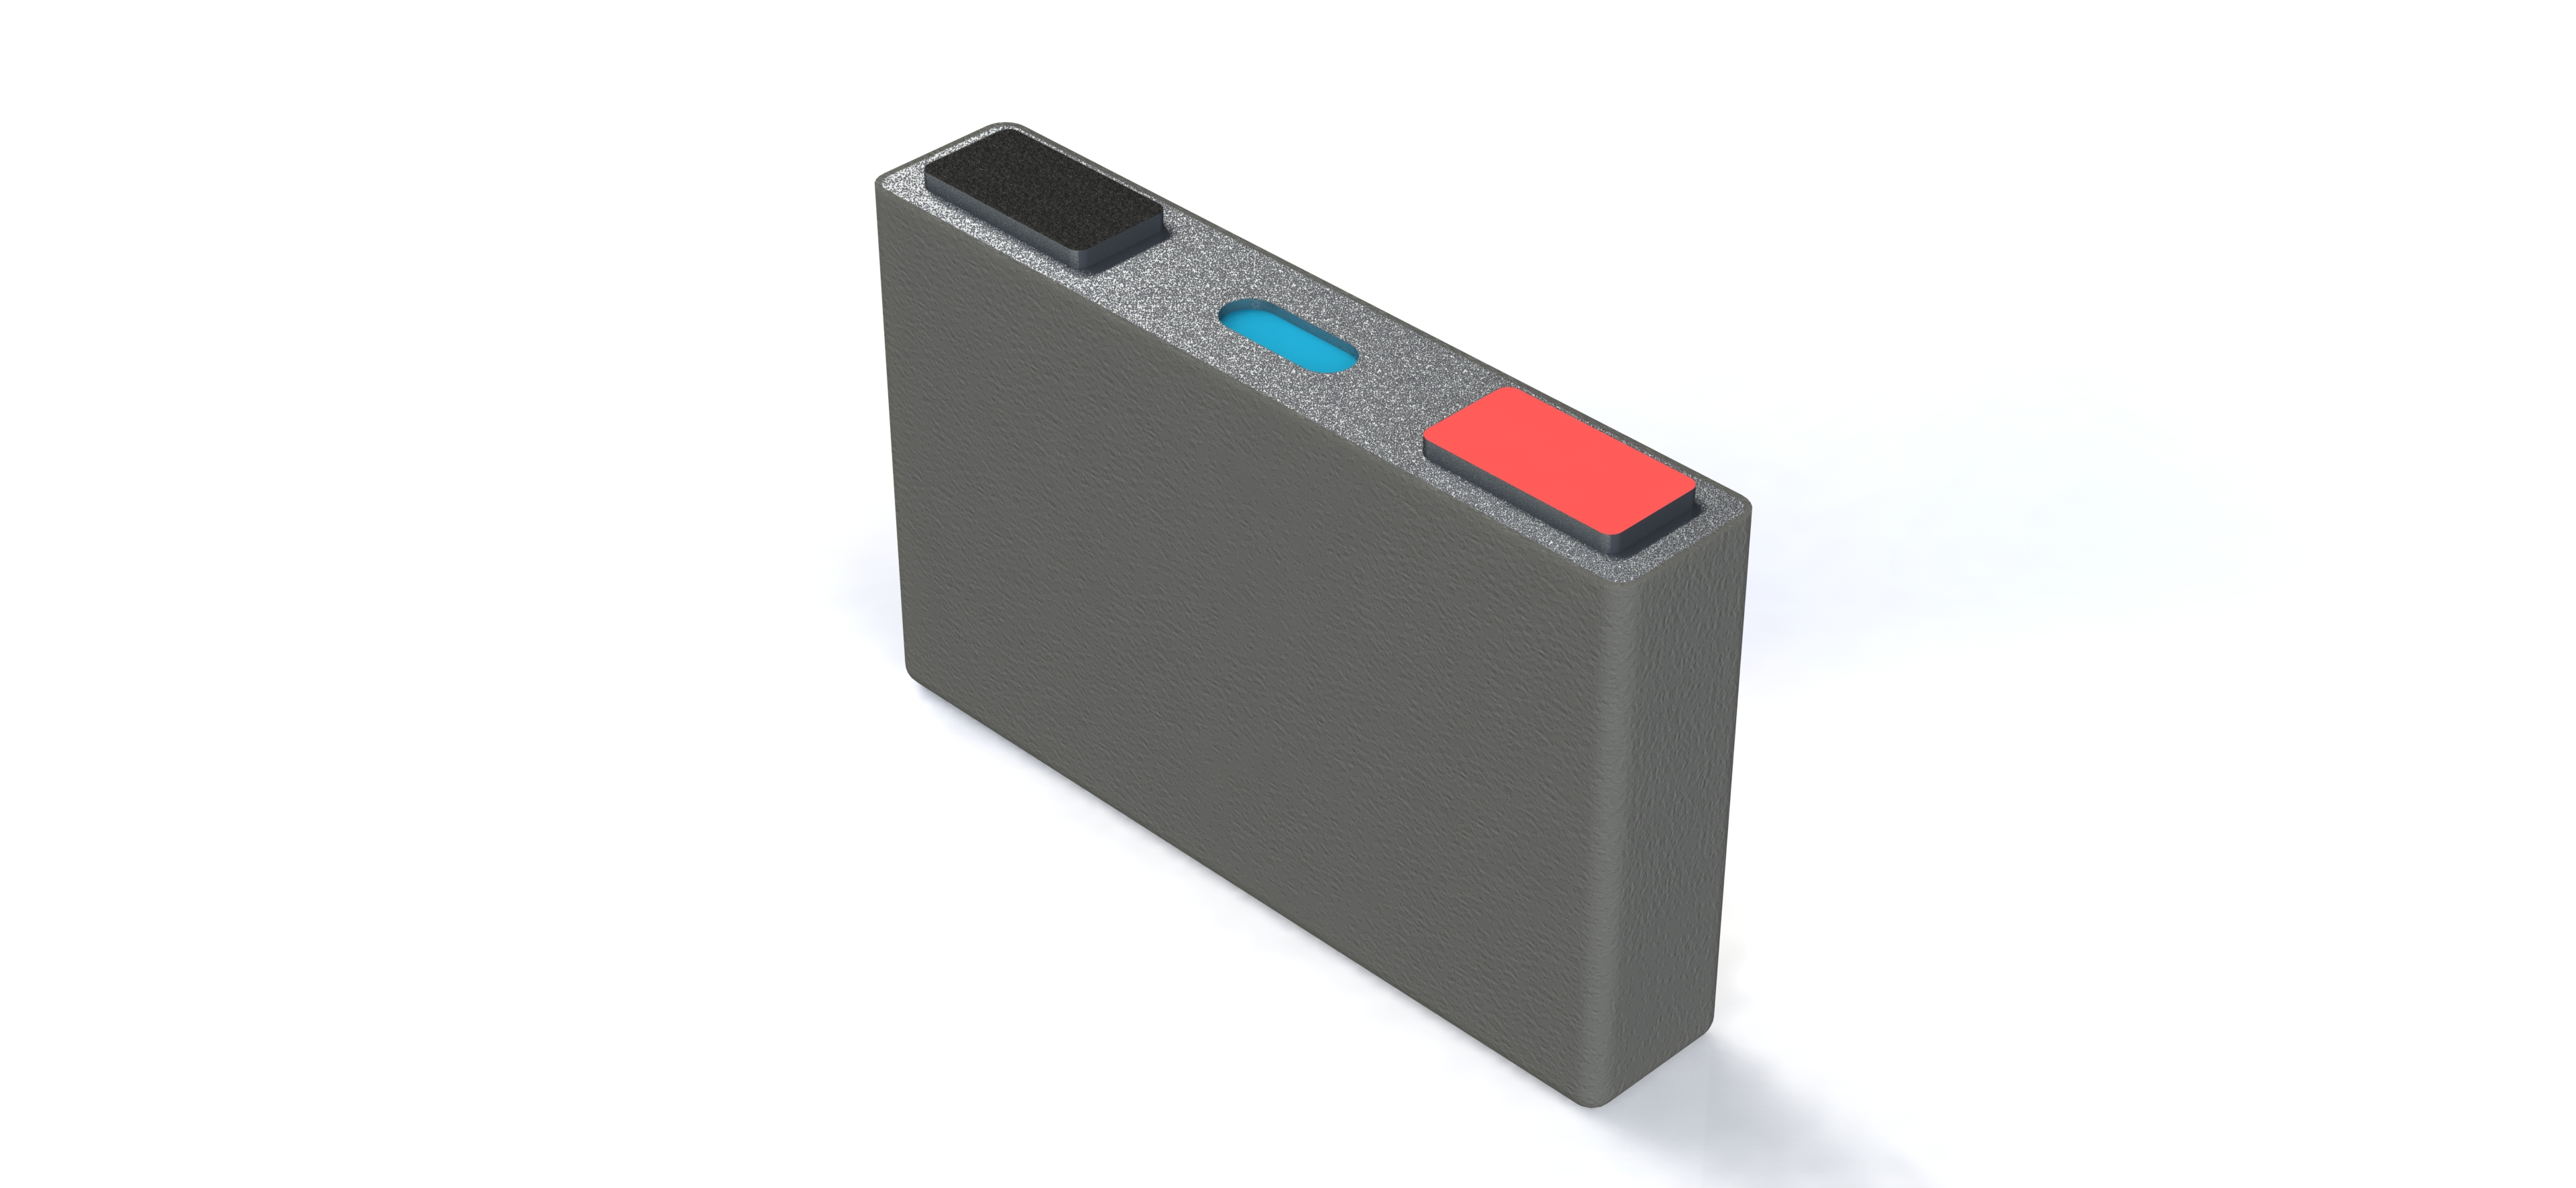
\includegraphics[width=0.9\textwidth]{figures/cell.jpg}
	\caption{电池单体设计}\label{fig:cell}
\end{figure}

在电池之间设置有电池间隔片,电池间隔片的设计阻止了电池在水平方向上的移动,并且在安装的时候可以控制间隔片的厚度来控制安装时的公差,便于手工的维修和安装,但是水平方向上安置的间隔片并没有阻止电池单体在垂直方向上的移动,在垂直方向上,本文的设计采用了一个电池箱压盖对于电池单体施加垂直压力,保证电池不会在垂直方向上发生跳动。

在电池单体之间的连接中,一般会使用铜排通过螺栓连接或者焊接与电池单体相连接,但是经过一段时间的的使用情况,螺栓通常会松动,产生危险因素,所以在目前的电动汽车电池箱设计中,一般是使用焊接方法连接电极端子 \cite{肖宁强2016插电增程式公交车电池系统设计}。

\section{电池模组级别的设计}

电池模组级别的设计主要关注的安全性问题是在模组内的电池热失控的控制和电池的压力出口点设计,电池压力出口点设计是当电池在发生热失控事件时,设计一个出口使得电池单体内部外泄的高温气流和物质沿着远离乘客的方向,或者任何会造成人员与财务损失的方向移动。这种方式会使车辆损坏和乘客安全风险最小化。在模组设计中,本文设计的压盖上有一个引导槽,可以起到泄出物质的引导作用,如图 \ref{fig:upholder} 所示。

\begin{figure}
	\centering
	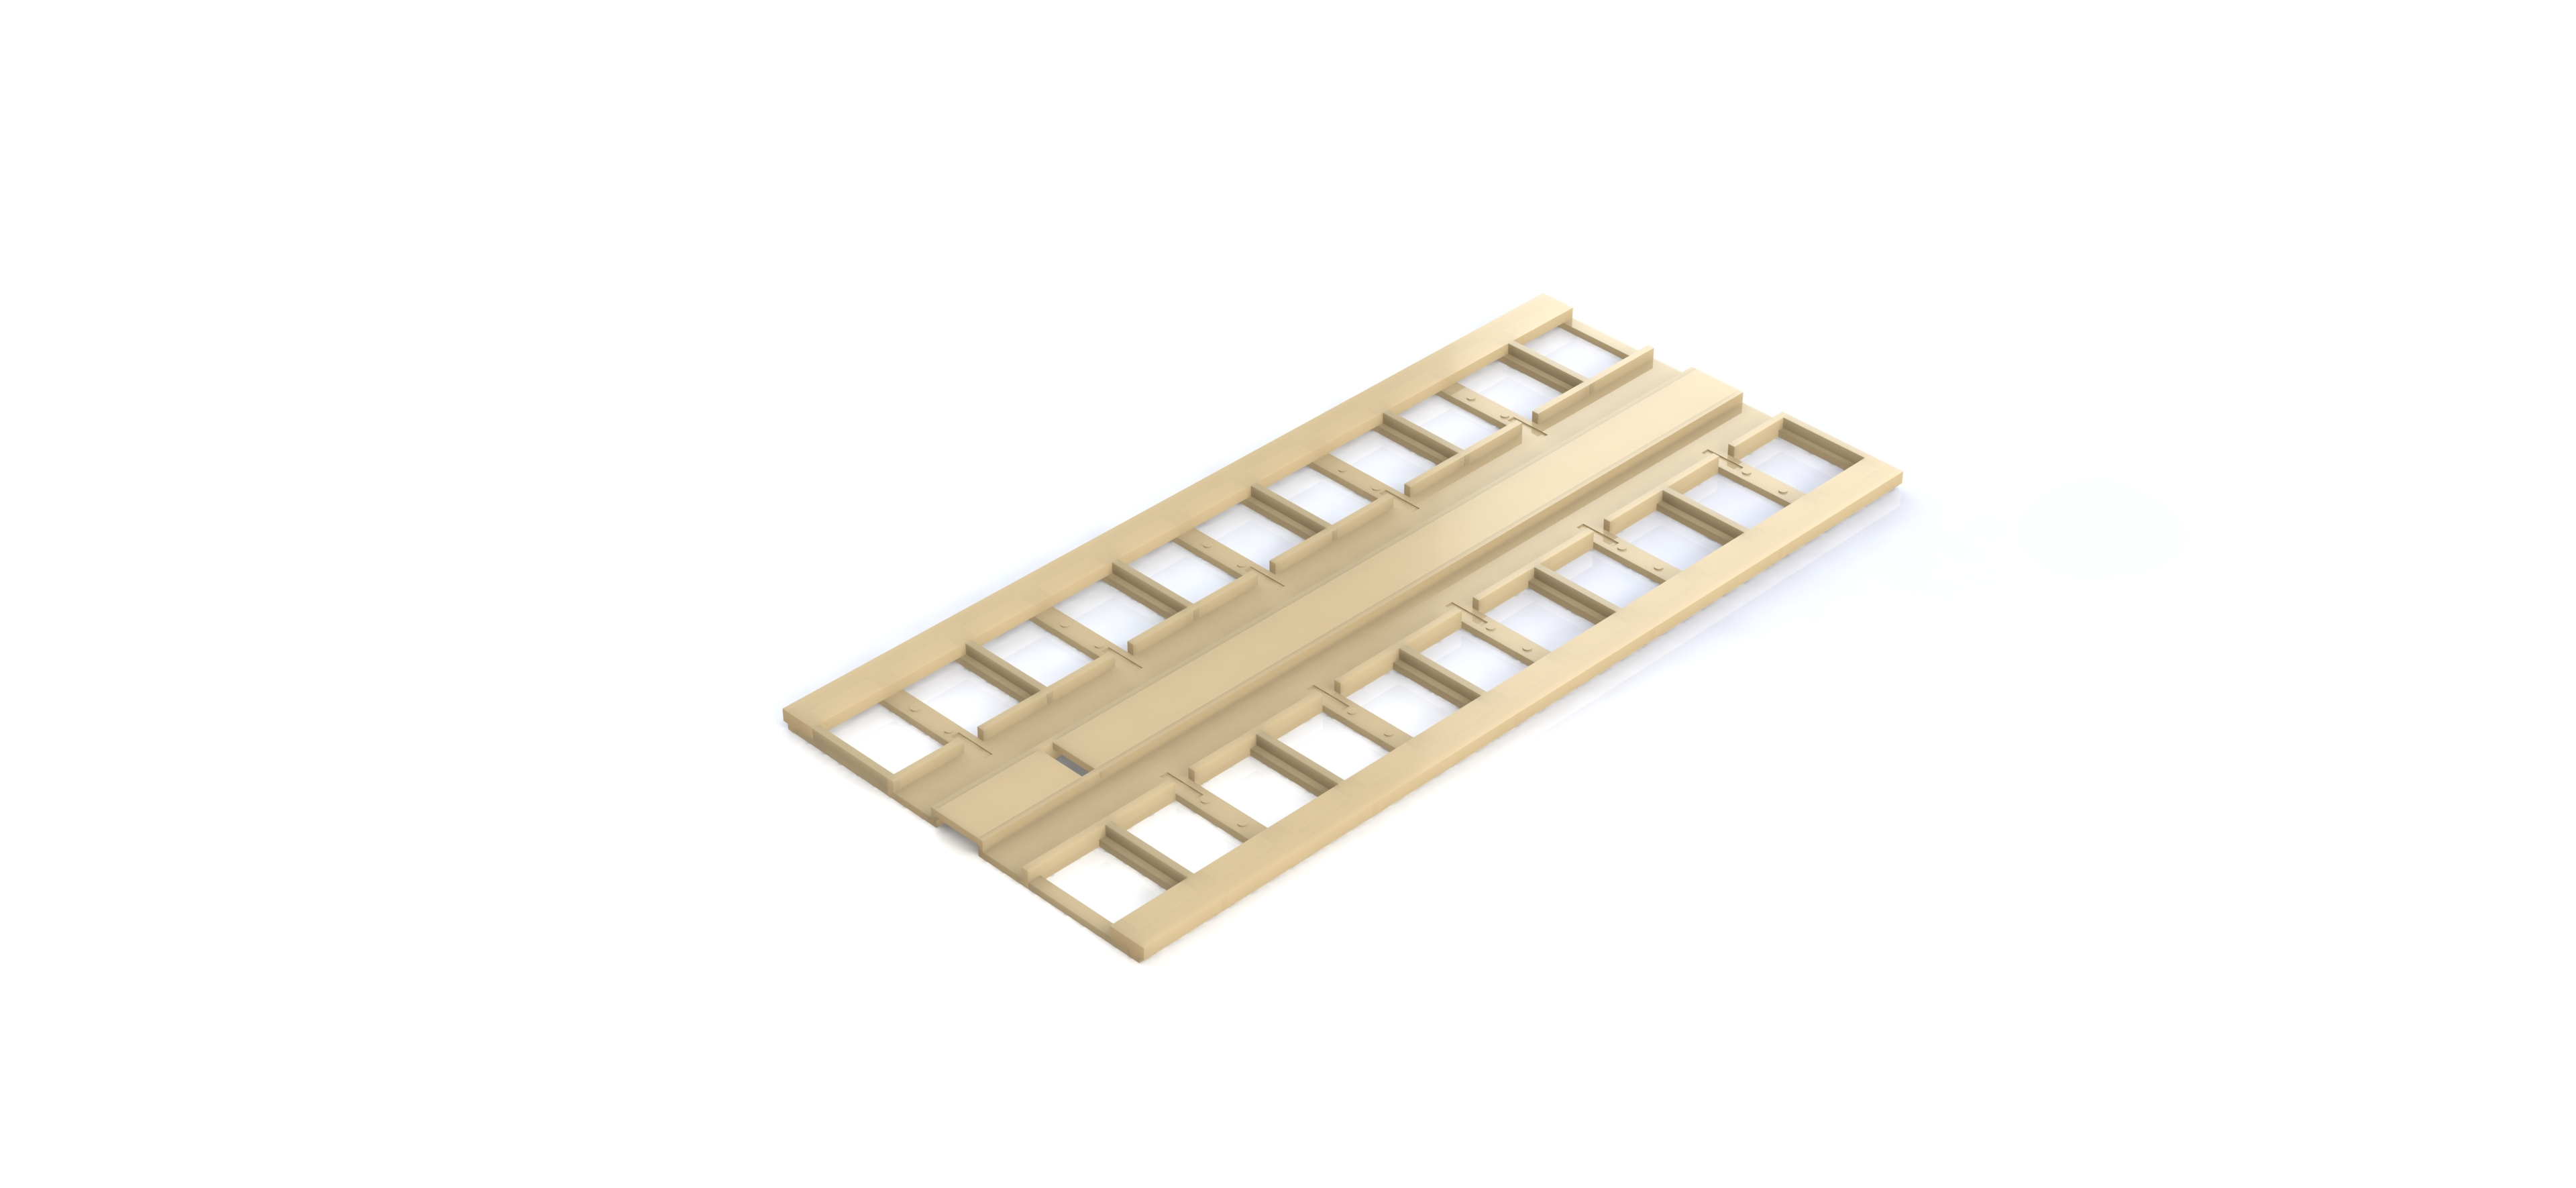
\includegraphics[width=0.9\textwidth]{figures/upholder.jpg}
	\caption{电池模组压盖设计}\label{fig:upholder}
\end{figure}

电池模组中压盖的材料为 PBT 工程塑料材质,由于 PBT 材料的耐热性较好,机械强度较大,材料的吸水性较低,尺寸稳定性好,故 PBT 材料被广泛应用于电气电子类,汽车工业类应用。每个在电池模组压盖的电池铜排下方有两个支撑住,可以起到支撑作用,由于电池连接的铜排上表面收到来自散热片压力的作用,该支撑柱可以提供支持力,避免连接铜排对电池极耳产生压力,损伤电池单体。

在电池的连接铜排上方贴有硅胶散热片,可以有效带走来自铜排的热量,并且与外壳相接触,起到绝缘和导热的作用 \cite{杨凯2014一种锂离子电池温控测试装置},选用硅胶片的原因是硅胶耐热性能较好,被广泛应用于电子器件起到导热作用,因为空气热阻较大,使用硅胶导热可以填充散热面的空气间隙,有效减小热源表面(铜排)和散热器件(外壳)之间的接触热阻。设计使用的导热硅胶片放置如图 \ref{fig:module} 所示,在该图中,在电池压盖上方已经安装好了连接铜排的和硅胶散热片。

\begin{figure}
	\centering
	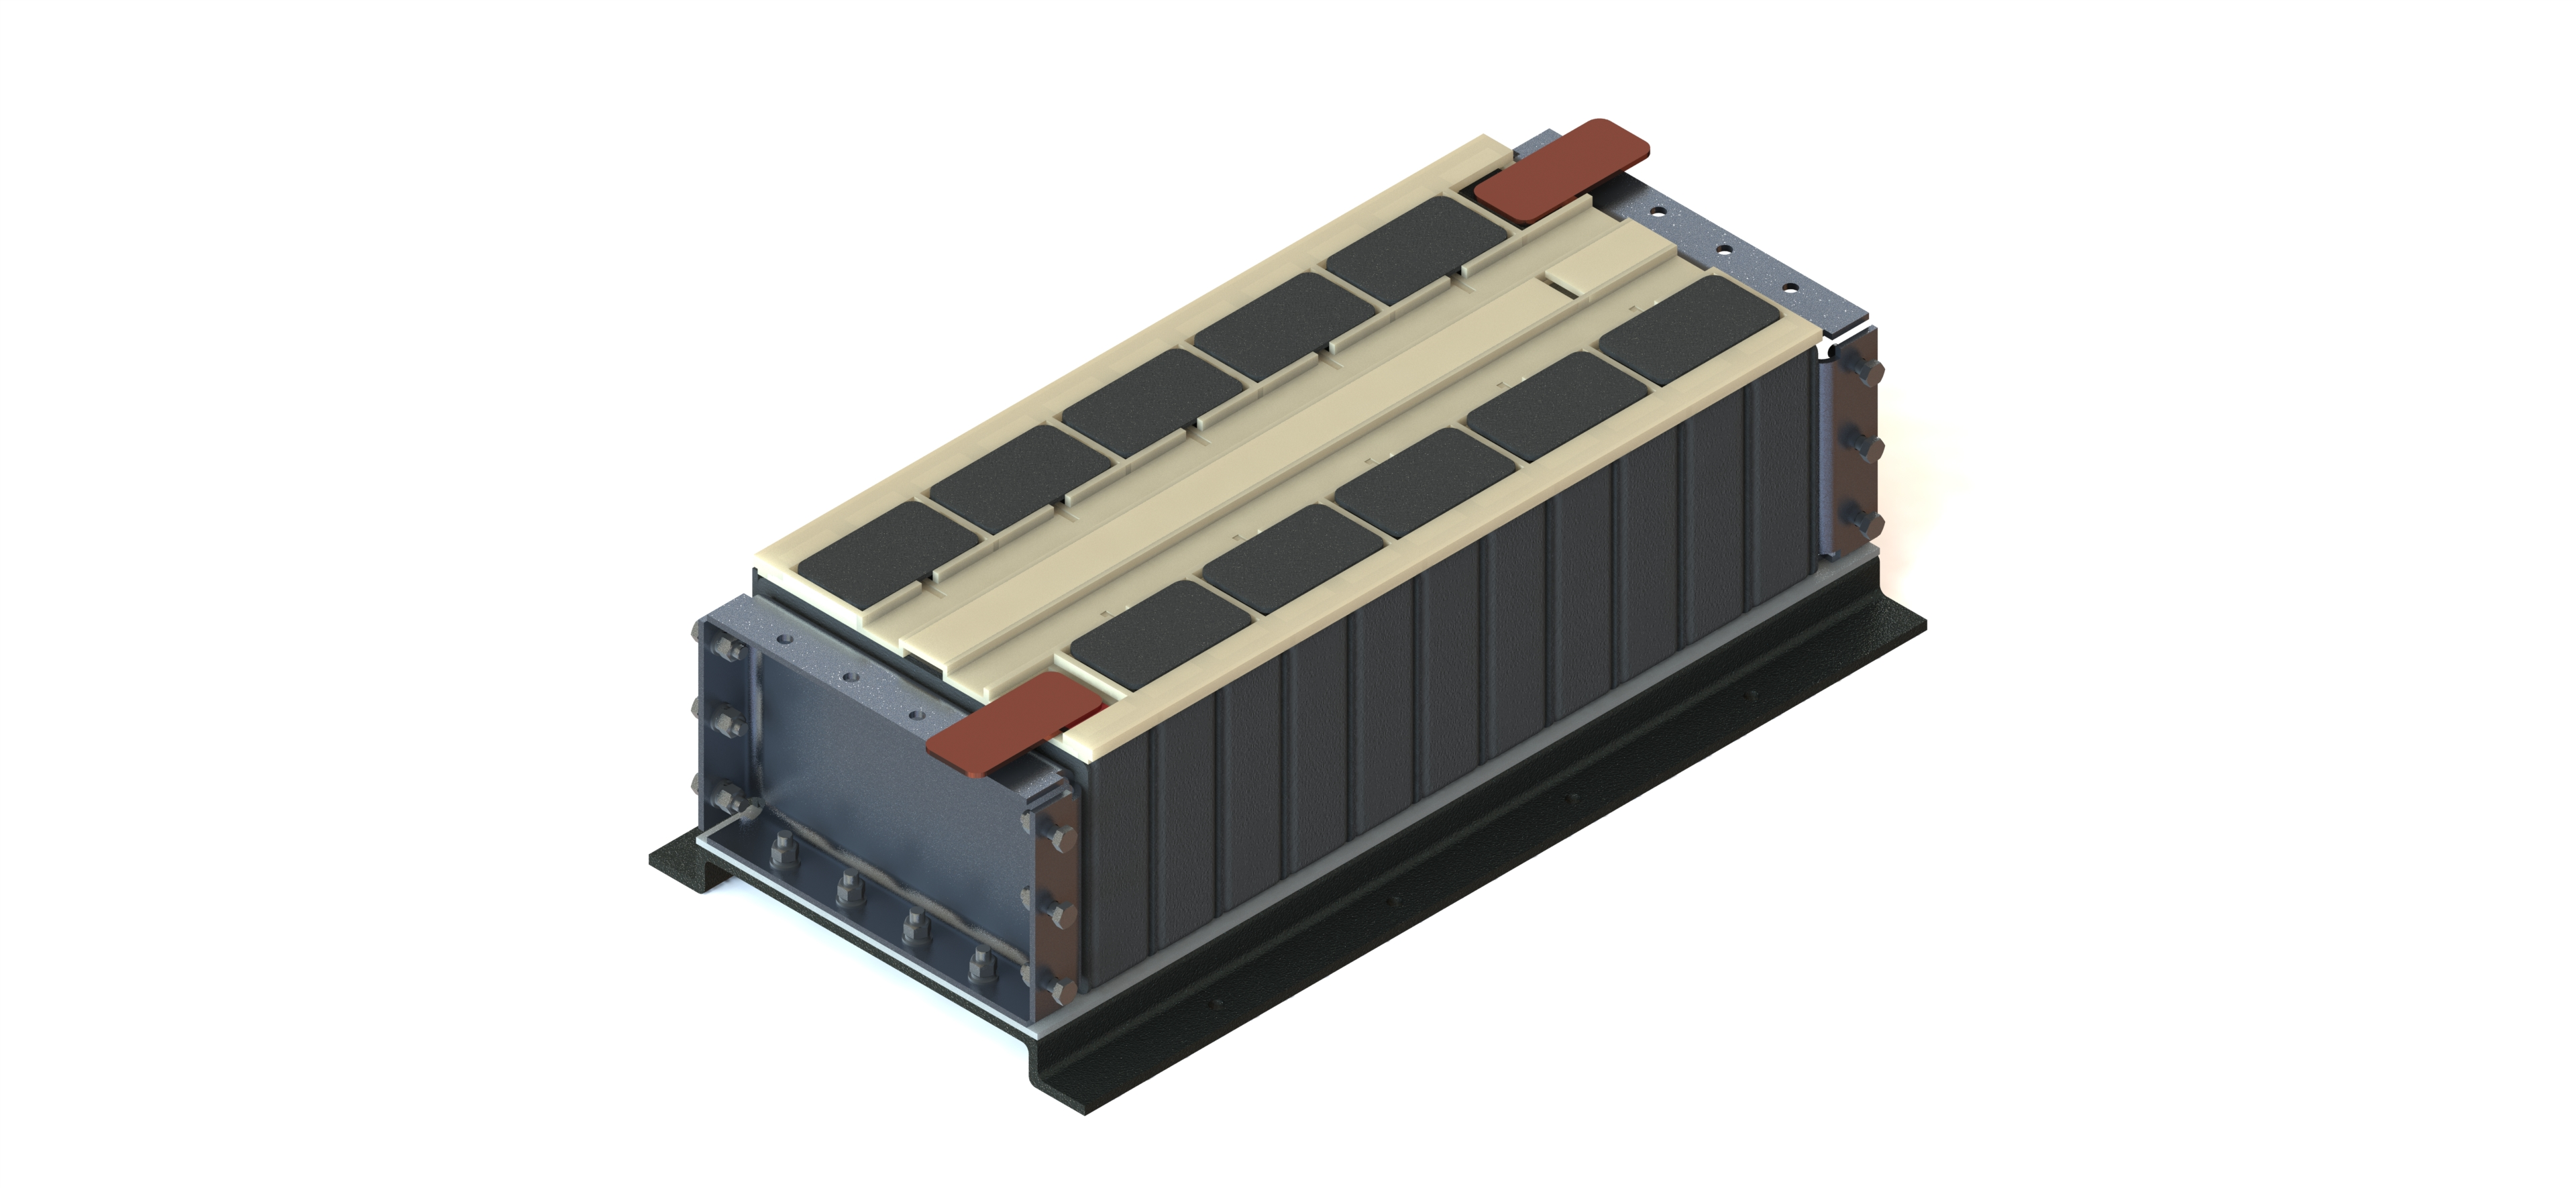
\includegraphics[width=0.9\textwidth]{figures/module.jpg}
	\caption{电池模组设计(无外壳)}\label{fig:module}
\end{figure}

电池模组的外壳为铝合金钣金材料,在外壳上方有两个凹槽,在一方面用于接触下方的硅胶散热片,将热量导出,在电池外壳该凹槽的上方可以安装水冷装置,带走热量。在电池模组的下方有漏网和凹槽,当电池发生漏液现象,漏出的液体会通过漏网流出,不会在电池模组内存留,以防止产生安全事故。含有铝合金外壳的完整的电池模组模型如图 \ref{fig:module2} 所示。

\begin{figure}
	\centering
	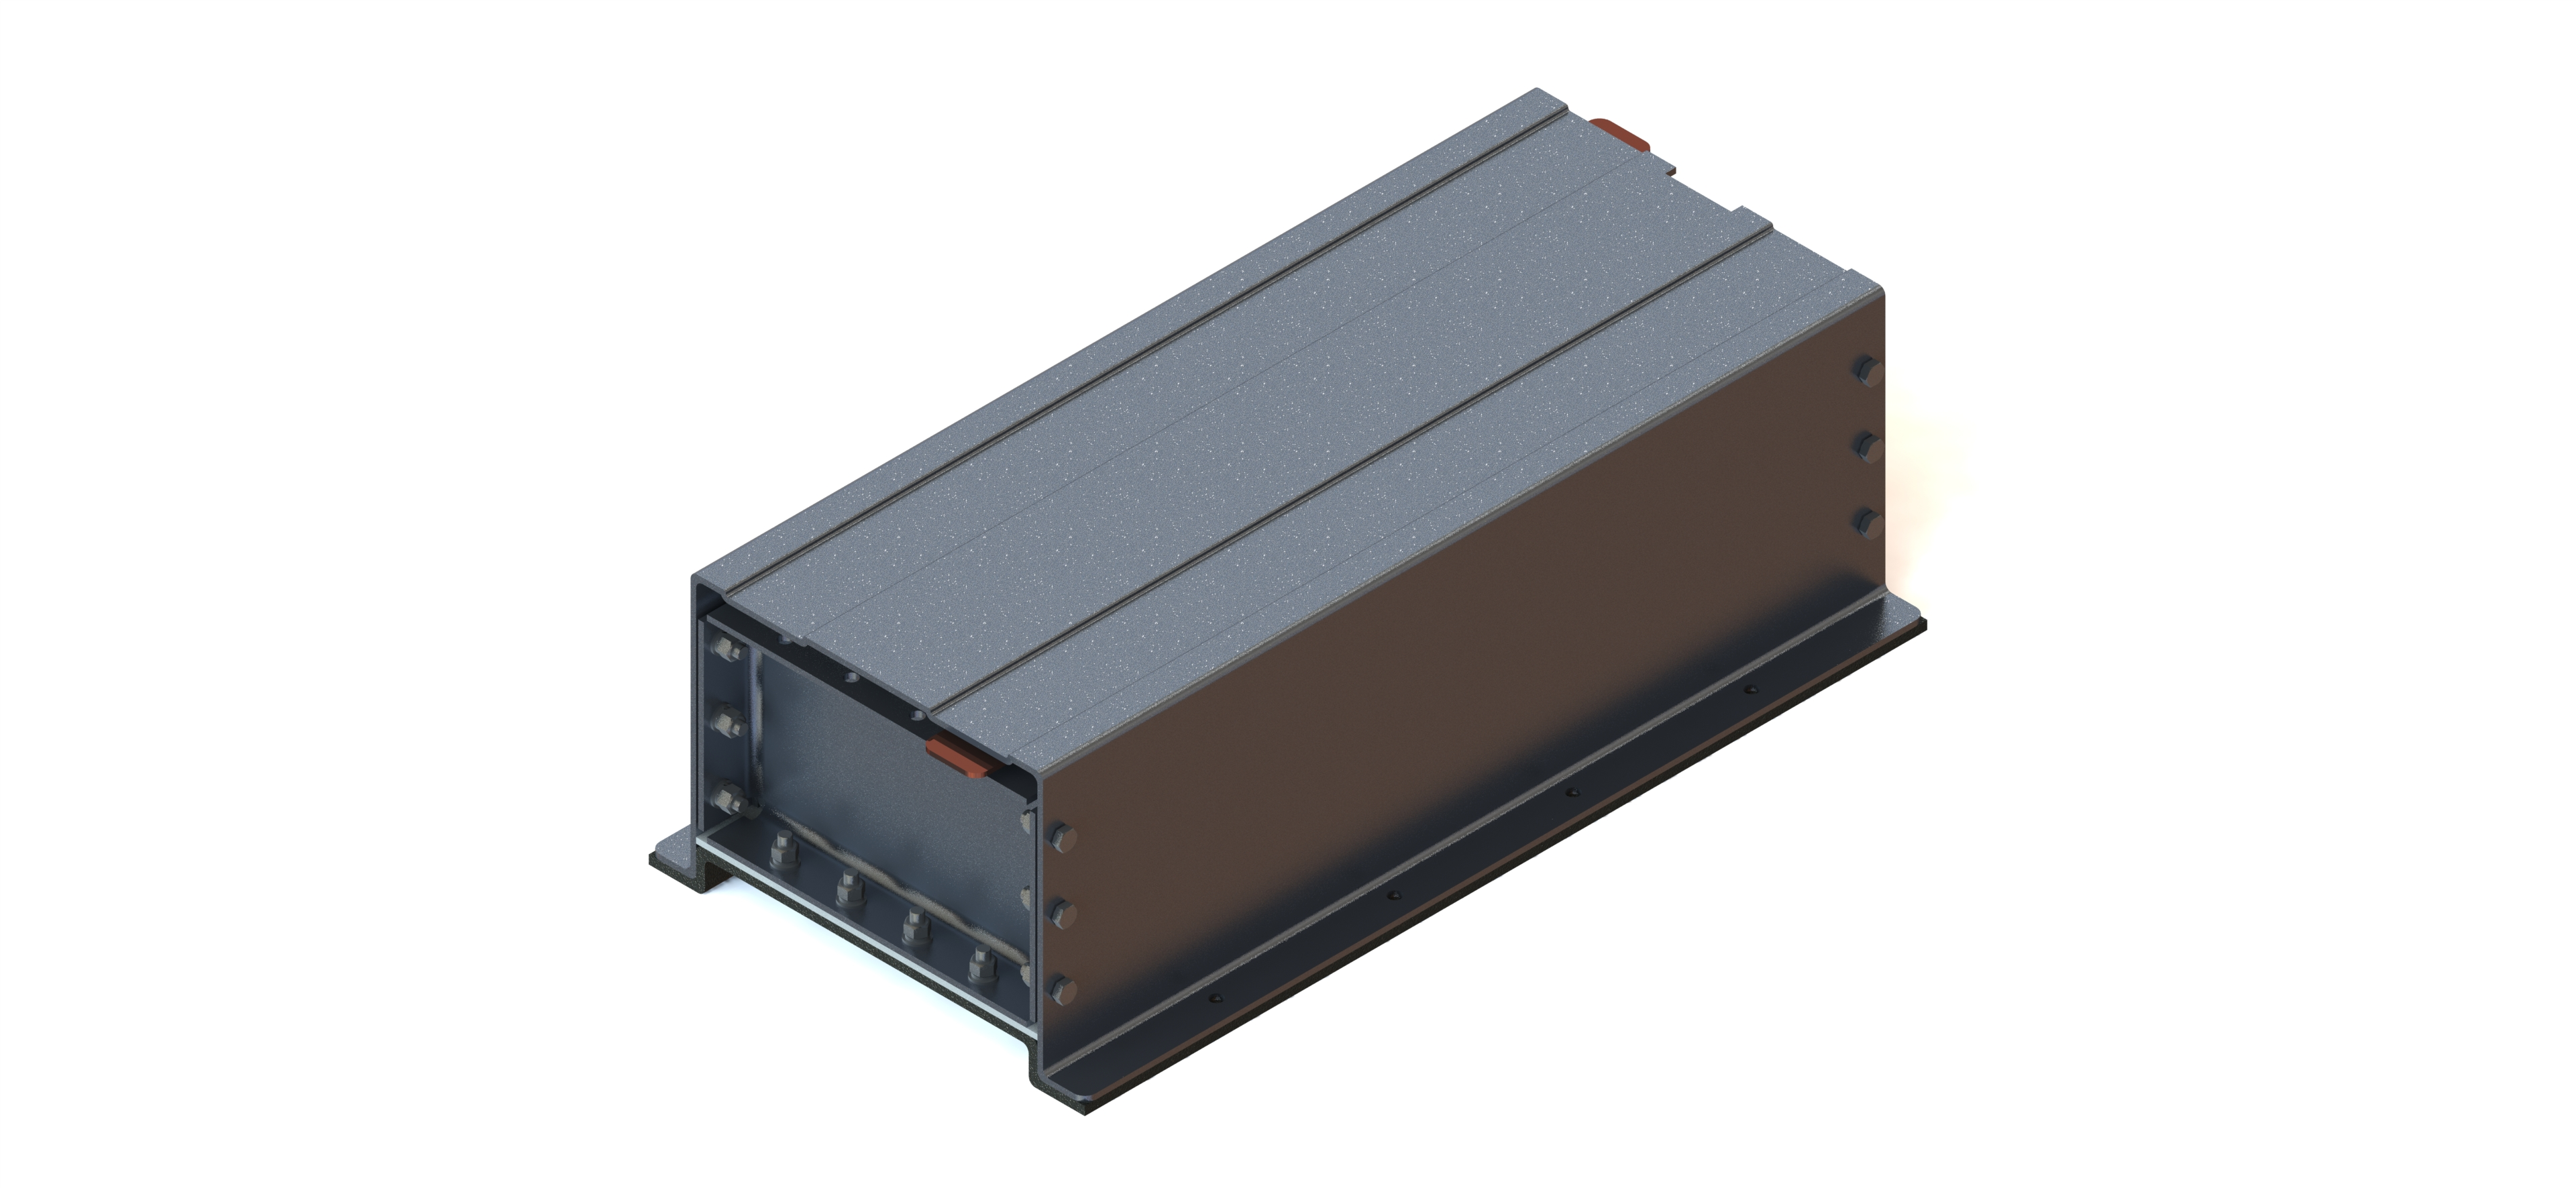
\includegraphics[width=0.9\textwidth]{figures/module2.jpg}
	\caption{电池模组设计(含外壳)}\label{fig:module2}
\end{figure}

\section{整体安装部分设计}
当考虑到电池箱与车体的连接部分,就不得不考虑车身振动和力的传递过程。当车辆在高速路以高速运行时,车辆会产生低频率的连续垂直振动输入;而当车辆运行在不平坦的道路上运行的时候,会产生冲击;当车辆起步或者转弯的时候,车辆会产生侧向加速度,而对于电池箱来说,会产生侧向力。

在美国专利 8642204 中提供了一种电池组安装框架的设计方案 \cite{BatteryManagementSystemUsedinElectricVehicles},它利用中空件结构接触电池组的下表面,并提供振动衰减的作用,在本文的设计中借鉴了该设计,使用了阻尼材料替代了专利中的结构,在电池箱的安装框架下方放置弹性阻尼橡胶板,以此来避免振动对于电池箱的影响。

在设计安装框架的时候,主要的问题是电池模组的安置问题,本文的设计参考了美国专利 8561743 中的设计方案,其设计了一种适合厂商修改电池模组数量的安装框架,并在不同的电池模组数量条件下,都能够保证电池箱的重量均匀分布,和较低的重心。本文使用了矩形的安装框架,安装框架被一根中梁等面积地分成两部分,在这两部分中,分别放置电池模组,电池模组的短边沿着车辆的纵向,长边沿着车辆的横向方向。这种电池模组的摆放方法会使电池箱的重量分布均匀,且安装稳固,如图 \ref{fig:Tray} 所示,该图展示了电池安装框架的结构。

\begin{figure}
	\centering
	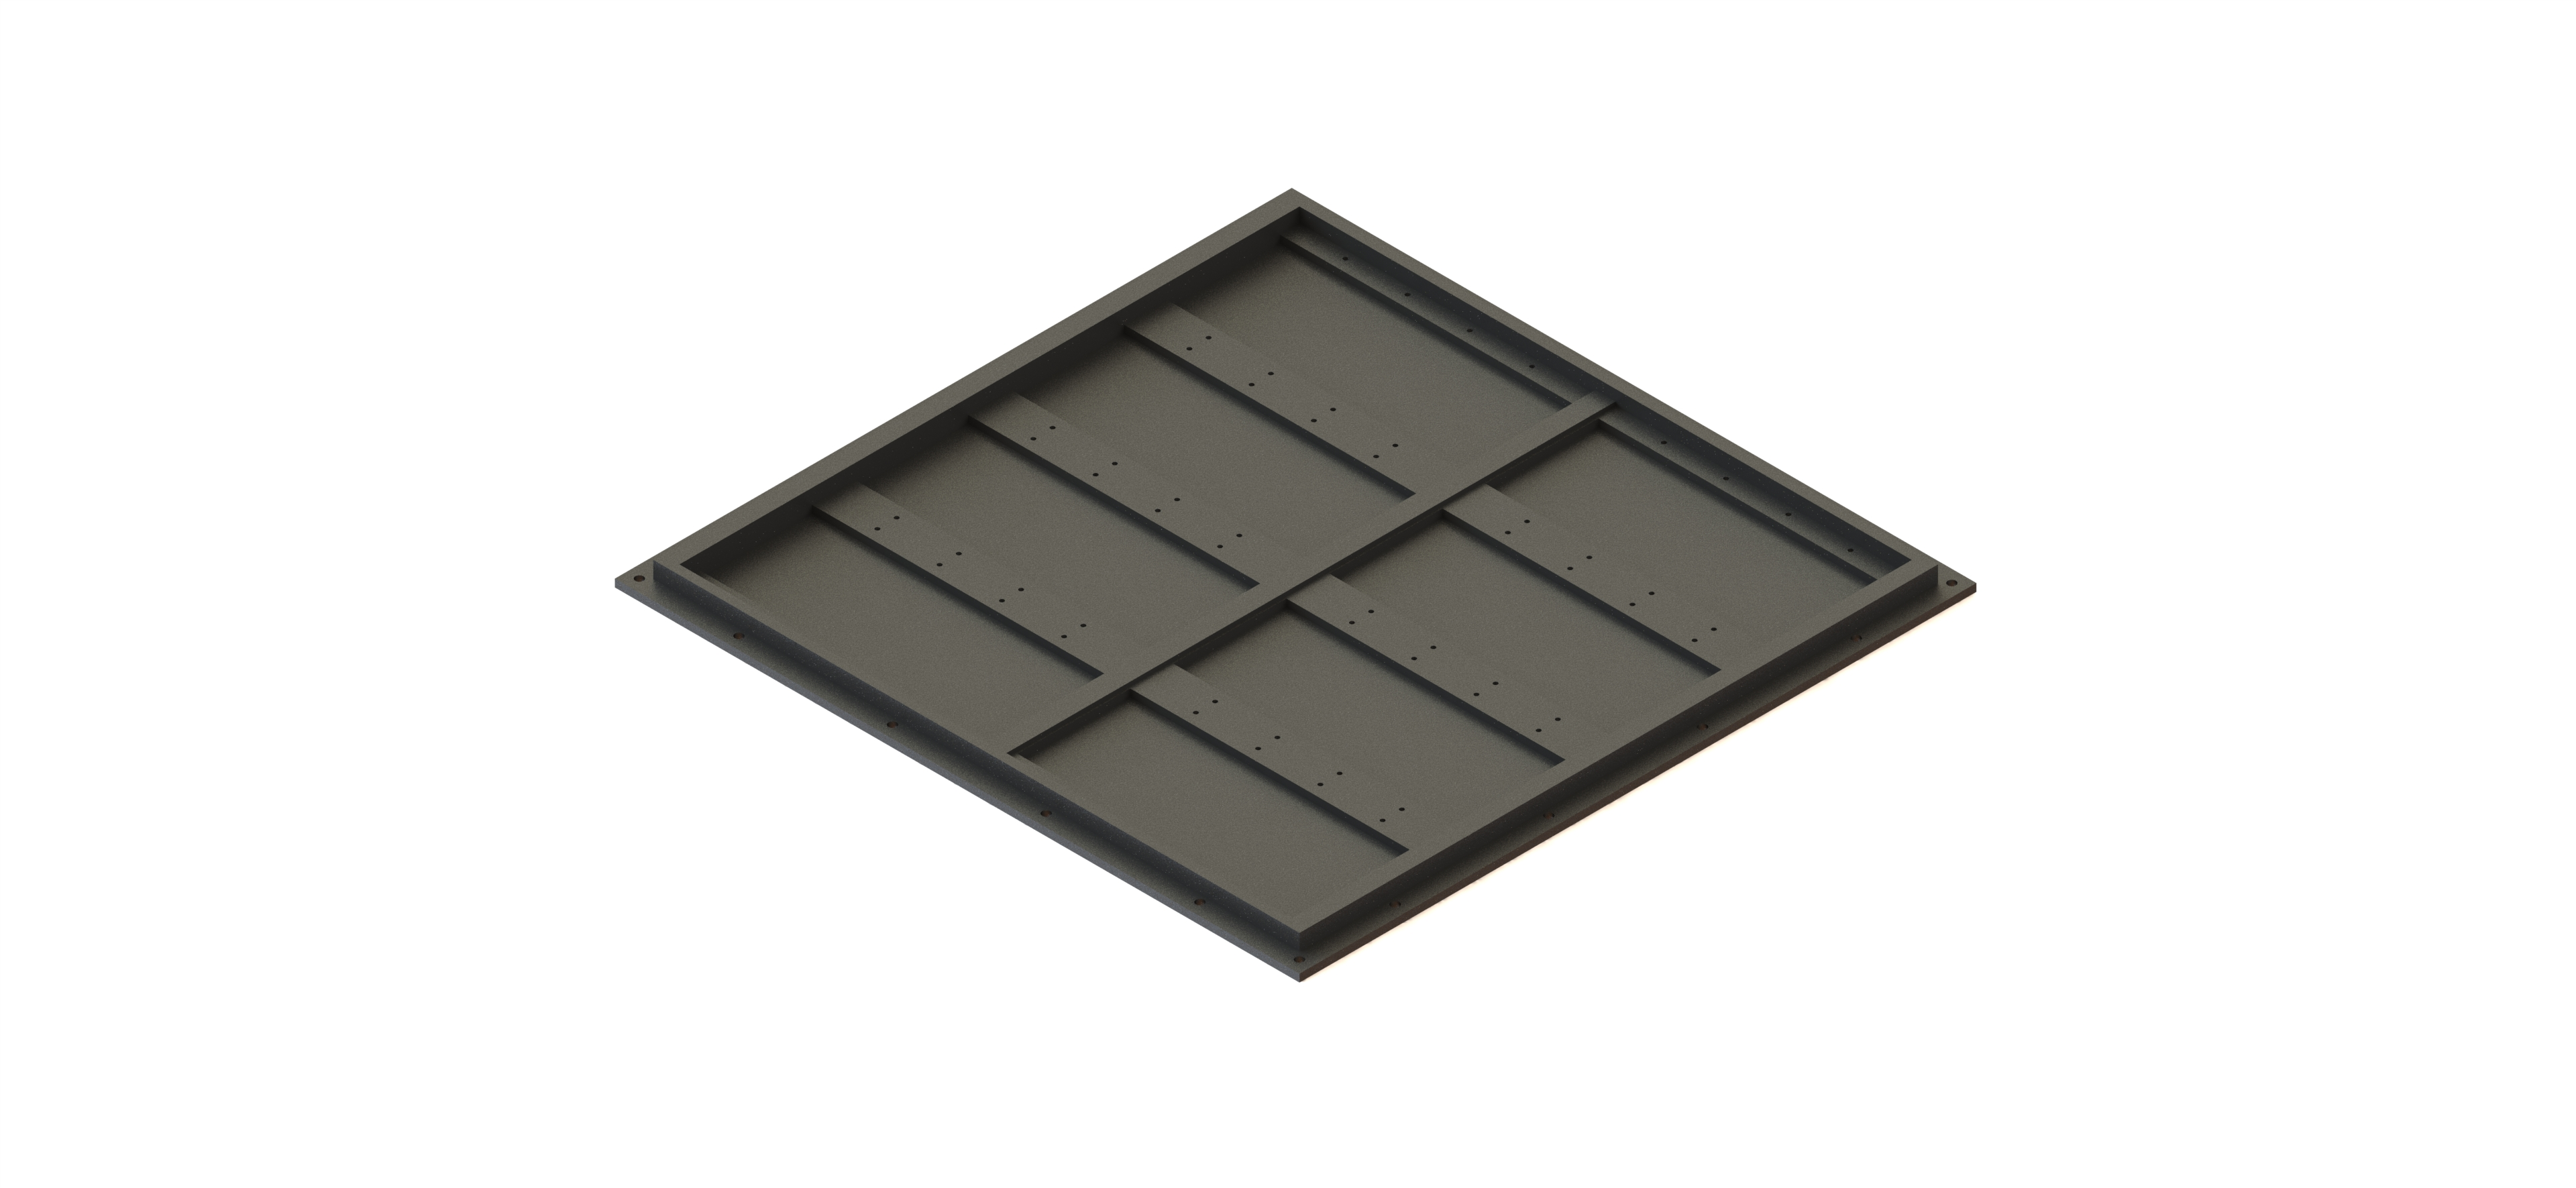
\includegraphics[width=0.9\textwidth]{figures/Tray.jpg}
	\caption{电池箱安装框架设计}\label{fig:Tray}
\end{figure}

设计最终的电池箱结构(不含上盖),如图 \ref{fig:Box} 所示,电池模组之间的连接采用铜线连接,铜线与模组之间的连接方式采用超声波焊接方式,不采用螺栓连接的方式。

\begin{figure}
	\centering
	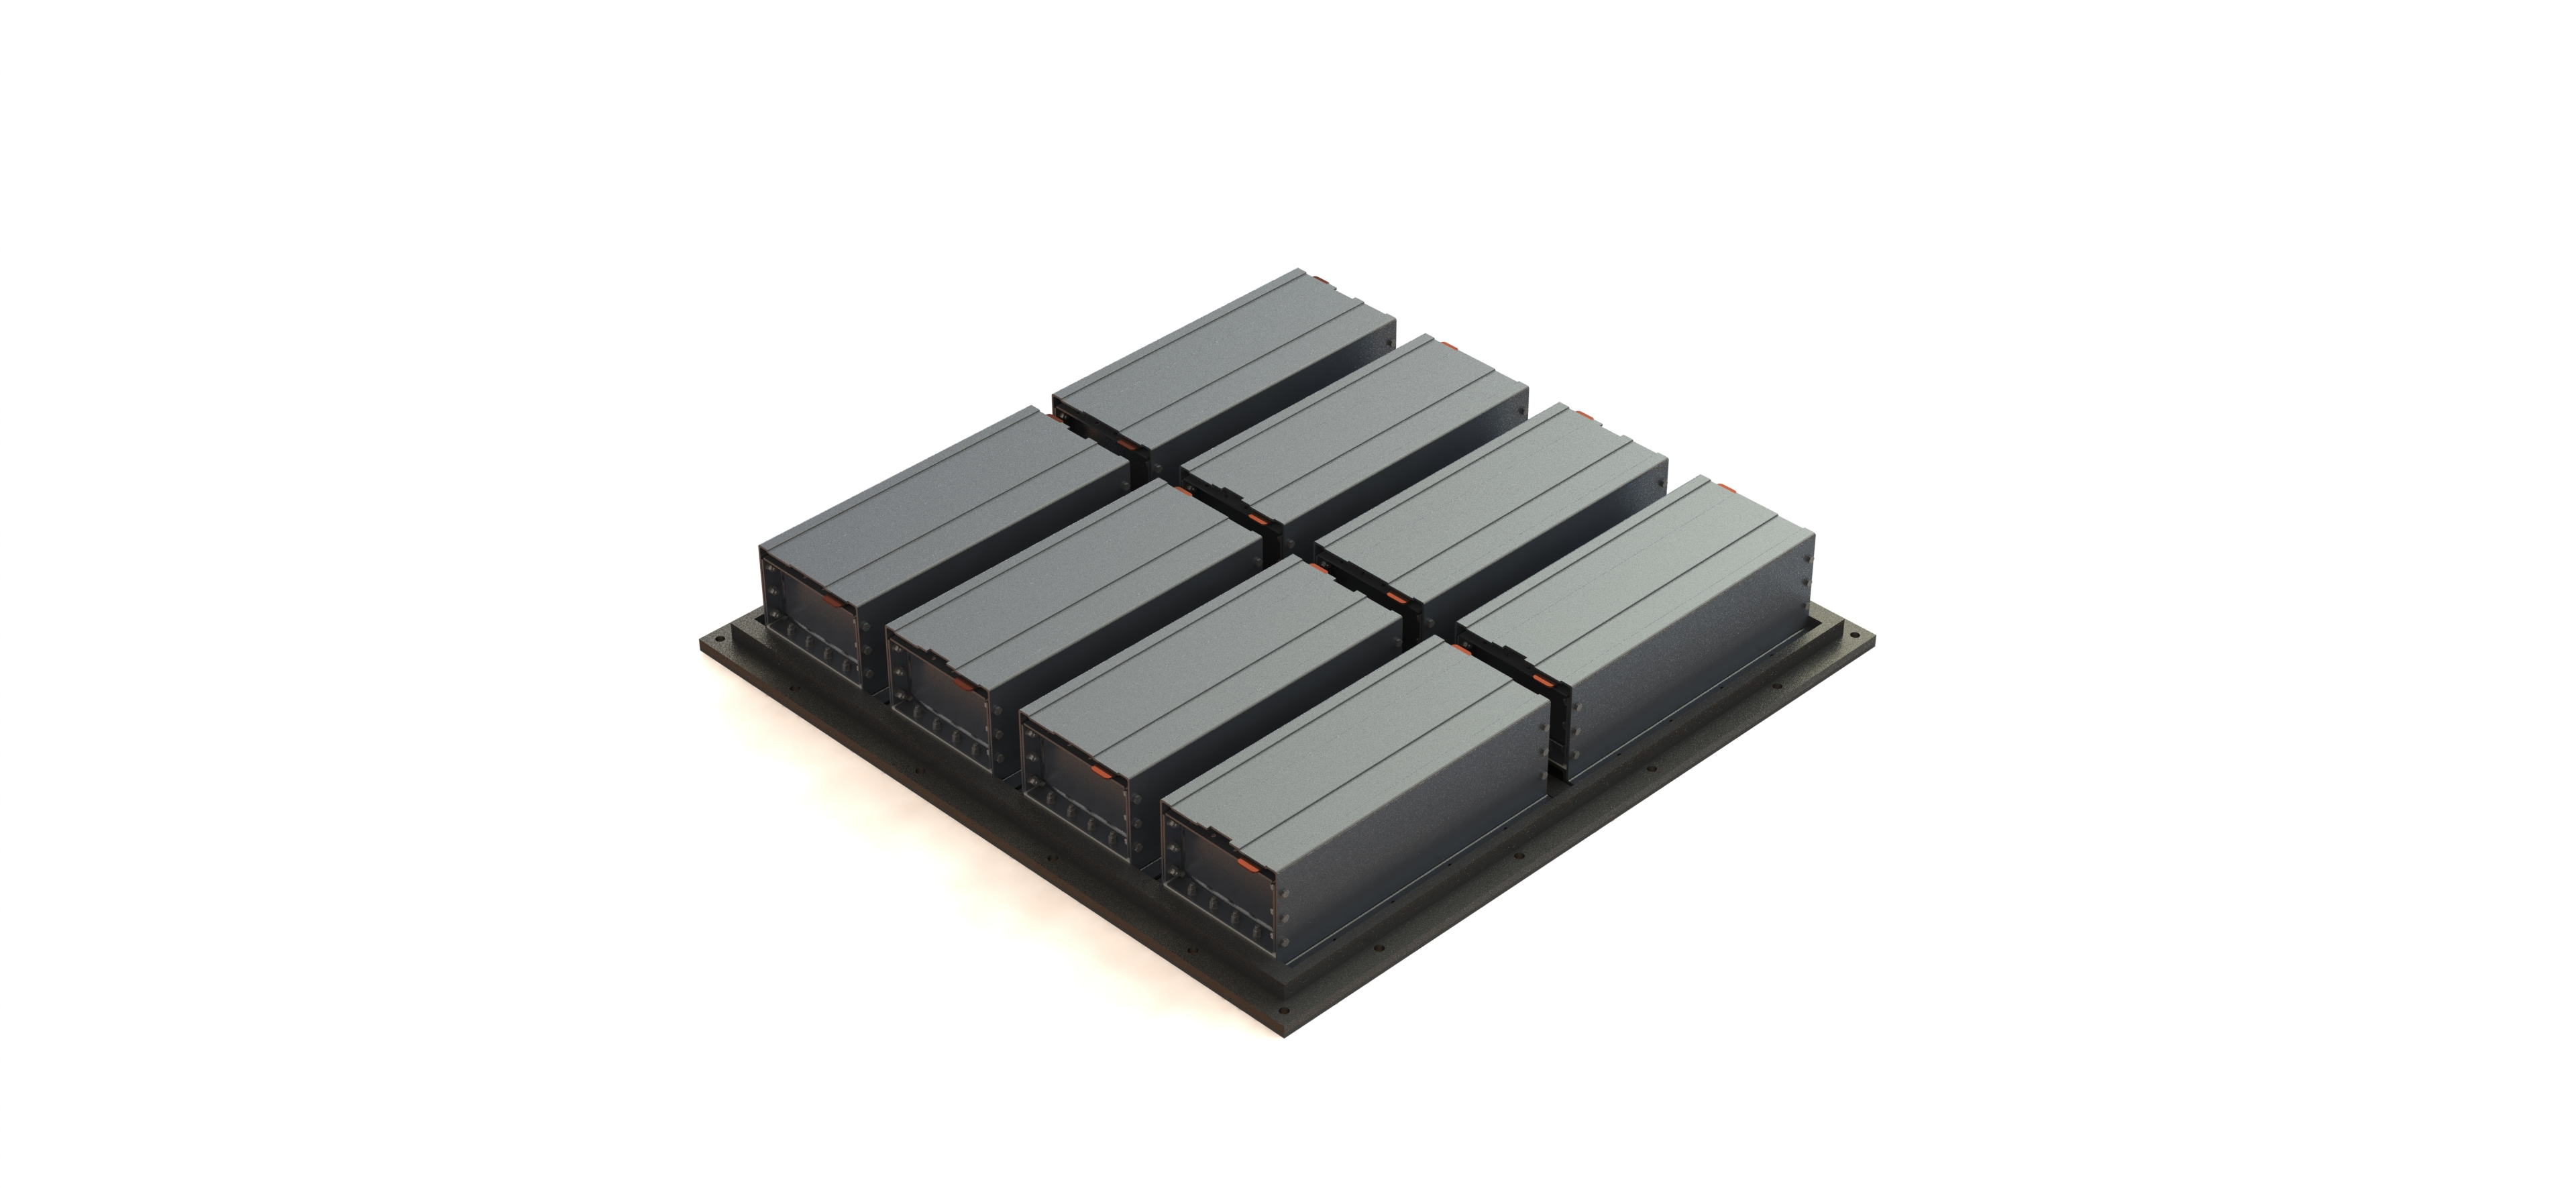
\includegraphics[width=0.9\textwidth]{figures/Box.jpg}
	\caption{电池箱整体设计}\label{fig:Box}
\end{figure}

设计完毕的电池箱机械参数如表 \ref{tab:mechinfo} 所示,表中的重量数据来自软件,是根据设计时采用的材料进行计算得到的重量值。

\begin{table}
	\centering
	\caption{电池箱机械参数} \label{tab:mechinfo}
	\begin{tabular*}{0.7\textwidth}{@{\extracolsep{\fill}}cc}
		\toprule
		参数项目			&数值		 \\
		\midrule
		质量/kg	     &115  \\
		长/mm     &891  \\
		宽/mm      &881\\
		高(不含外壳)/mm     &142  \\
		\bottomrule
	\end{tabular*}
\end{table}

\subsection{热管理}
在本文的设计当中,并未设计电池箱的热管理系统,但是在第三章节设计电池模组的过程当中,给该电池箱的热管理系统的设计准备了设计的方法。

在混合动力汽车在使用纯电动模式行驶时,由于本文设计的电池箱的额定功率和实际的驾驶功率相接近,在车辆日常行驶时,车辆的电池箱放电的倍率较大。传统风冷技术是根据气体对流换热方式进行电池箱的主动散热的,该方案的成本较低,在设计的时候较为简单,但是风冷散热的散热量有限,在电池箱的密集放热部位,如电芯和极耳等位置,使用风冷散热无法做到及时带走热量,这会导致电池箱内部的温度分散不均,影响电池的寿命,另外一方面,电池箱发生危险时,如电池箱发现热失控现象,风冷无法做到对于危险的控制。

而在其他的散热方案中,传统的液冷技术应用于电池箱方面会导致一些危险,如液体管路泄漏和阻塞,而且在日常的使用当中,传统液冷方案需要经常更换冷却液,否则在管路内产生沉积,而且系统的重量较大,占据空间较大。而采用固体相变技术散热的方案实现混合动力电池箱散热,因为固体相变技术较为复杂,而且目前的研究尚且不成熟,采用该方案的散热系统控制难度较大,而且该方式采用的合金散热材料无法做到良好的绝缘性。因此,本文设计中采用的散热方案是采用热管散热,通过安置在电池模组上方的热导管,及时带走箱内的热量。

热管散热是采用了液体发生气-液相态变化时生成和吸收热量的原理设计的,在热管的内部被分为三段,三段中的物质可以互相流通。第一段是蒸发段,贴着需要散热的表面,蒸发段内的液体吸收热量后蒸发汽化,通过第二段绝热段,到达第三段冷凝段,在冷凝段高温气体与外界交换热量,放出热量,冷凝成为液体流回第一段 \cite{周海阔2017基于热管技术的锂电池箱热管理系统设计与实验验证}。通过这种简单循环散热机制,可以做到较好的热传导速率,并且体积较小,适合在混合动力电池箱内使用。

在电池模组的下方预留了一部分空间 ,可以安装用于加热使用的电阻丝,在电池管理系统中,可以通过电池箱内部的散热和加热控制,可以有效地将箱内的环境温度差异降低,保证电池的工况条件一致性,提高电池的寿命 \cite{叶欣2017电动汽车锂离子电池散热加热设计}。

\subsection{振动隔离}
在本文的计算校核中使用了一种较为简单的校核方式,也即是利用车身的加速度来计算电池箱在运动时所产生的最大加速度量的计算方式。而在实际的驾驶过程中,由于路面存在不平度频率输入,故在设计的时候需要考虑电池箱内部的连接结构和支撑结构因为振动所造成的影响,因为在驾驶过程中的电池箱瞬时振动可能会导致电池箱因此产生的加速度远远大于本文所假设的稳态加速度条件。

在之前的机械设计章节,本文对于电池箱单体的振动隔离采用的是在水平方向上的隔板吸收振动的能量,在垂直方向上使用电池模组的压盖来抑制垂直方向上的振动。而在整体的安装方面上本文参考了美国专利 8642204 中的抗振动电池箱安装框架设计,在安装电池箱的底座四周安装阻尼块来实现振动的隔离。

\section{设计校核}

在本设计中主要的校核内容被分为两类,一类是静态校核,一类是动态校核,由于电池箱与车辆底盘相连,故车辆的运行状态会影响电池箱的受力状态,仅仅考虑电池箱在静态状态下的受力状态的校核是不可靠的,因为电池箱的质量较大,在运动过程中若存在加速度,将会对电池箱连接结构产生力的作用 \cite{王文伟2016电动汽车电池箱结构随机振动疲劳分析}。

\subsection{水平方向}
在汽车行驶过程中,汽车的加速和减速会造成汽车在水平方向上存在加速度;汽车的转向过程中,汽车会产生侧向的加速度。而汽车的纵向加速度和横向加速度的大小取决于汽车的运动状态。

在这里,本文计算的汽车的纵向加速度分为两类,一类为汽车加速运行时的纵向加速度,一类是汽车踩下刹车时,汽车减速运动的加速度。在目前的技术情况下,汽车加速时的加速度一般不会超过 1G(一个重力加速度的大小),该加速度的大小相当于百公里加速时间 2.8 秒,而当汽车踩下刹车时,车辆的最大减速度也不会超过 1G(一个重力加速度的大小)。

汽车的横向加速度与车辆的转向半径和汽车的转向速度有关,由于一般汽车的质心高度较高,质心并不与路面重合,在汽车的横向加速度超过一定值时汽车会发生侧翻现象,如式 \ref{equ:fanche} 所示,该式中,$a$ 为车辆的横向加速度,$m$ 为车辆的质量,$L_2$ 为车辆的轮距,$L_1$ 为车辆的质心高度,$g$ 为重力加速度。

\begin{equation}
\begin{aligned}
	\label{equ:fanche}
	(m \times a)\times L_2 &> (m \times g) \times \frac{L_1}{2} \\
	a &> \frac{g\times L_1}{2 \times L_2}
\end{aligned}
\end{equation}

根据一般车辆的数据带入计算,车辆发生侧翻时的最大加速度一般不超过 2G,也就是说,车辆在正常行驶的时候,理论的最大的横向加速度不超过 2G。

根据以上的计算过程,据此可以估计车载电池箱的最大水平加速度不超过 2G,根据这个加速度的边界值来判断电池箱的连接螺栓的强度。

电池底座上的螺栓连接采用紧螺栓连接,在安装的时候需要拧紧螺栓。当安装完毕的时候,螺栓的螺纹部分受到的力分为两类,一类是在安装时候施加的预紧力的 $F_t$ 产生的拉伸应力的作用,还有一类是因为在螺纹接合面处由存在的螺纹副阻力矩 $T_1$ 而产生的扭转切应力。

根据计算公式,该类型(紧螺栓连接)的螺栓在危险截面存在的拉伸应力的大小为:

\begin{equation}
	\sigma = \frac{F'}{\frac{\pi}{4}d_1^2}
\end{equation}

该类型(紧螺栓连接)螺栓危险截面的扭转切应力为:

\begin{equation}
	\tau=\frac{T_1}{W}=\frac{F'tan(\lambda+\rho_v)\frac{d_2}{2}}{\frac{\pi}{16}d_1^3}=tan(\lambda+\rho_v)\cdot \frac{2d_2}{d_1} \cdot \frac{F'}{\frac{\pi}{4}d_1^2}
\end{equation}

式中的 $T_1$ 为电池箱螺栓的扭转力矩,$W$ 为螺栓抗扭截面系数,$F'$ 为螺栓的预紧力,$\lambda$ 为电池箱螺栓的螺纹升角,$\rho_v$ 为电池箱螺栓的当量摩擦角,$d_2$ 为电池箱螺栓的螺纹中径,$d_1$ 为电池箱螺栓的小径。本文使用的是常用的 M10 型号 GB 钢制普通螺栓,带入 $tan\rho_v \approx 0.17$,$\frac{d_2}{d_1} \approx 1.04 ~ 1.08$,$tan\lambda \approx 0.05$ 代入得到:

\begin{equation}
	\tau \approx 0.5 \sigma
\end{equation}

由于螺栓的材料存在塑性,根据第四强度理论来确定螺纹部分的应力:

\begin{equation}
	\label{equ:1.3}
	\sigma_{ca}= \sqrt{\sigma^2+3\tau^3}=\sqrt{\sigma^2+3(0.5\sigma)^2}=1.3 \sigma
\end{equation}

可以看出,虽然对于本文使用的螺栓受到了拉伸力和扭转力的作用,但是在计算的时候仍可以按照纯拉伸的螺栓来计算强度,在计算中,仅仅需要将所受到的拉力,在电池箱中,拉力即为预紧力,增大 $30\%$,就足以包括扭转的影响。

\begin{figure}
	\centering
	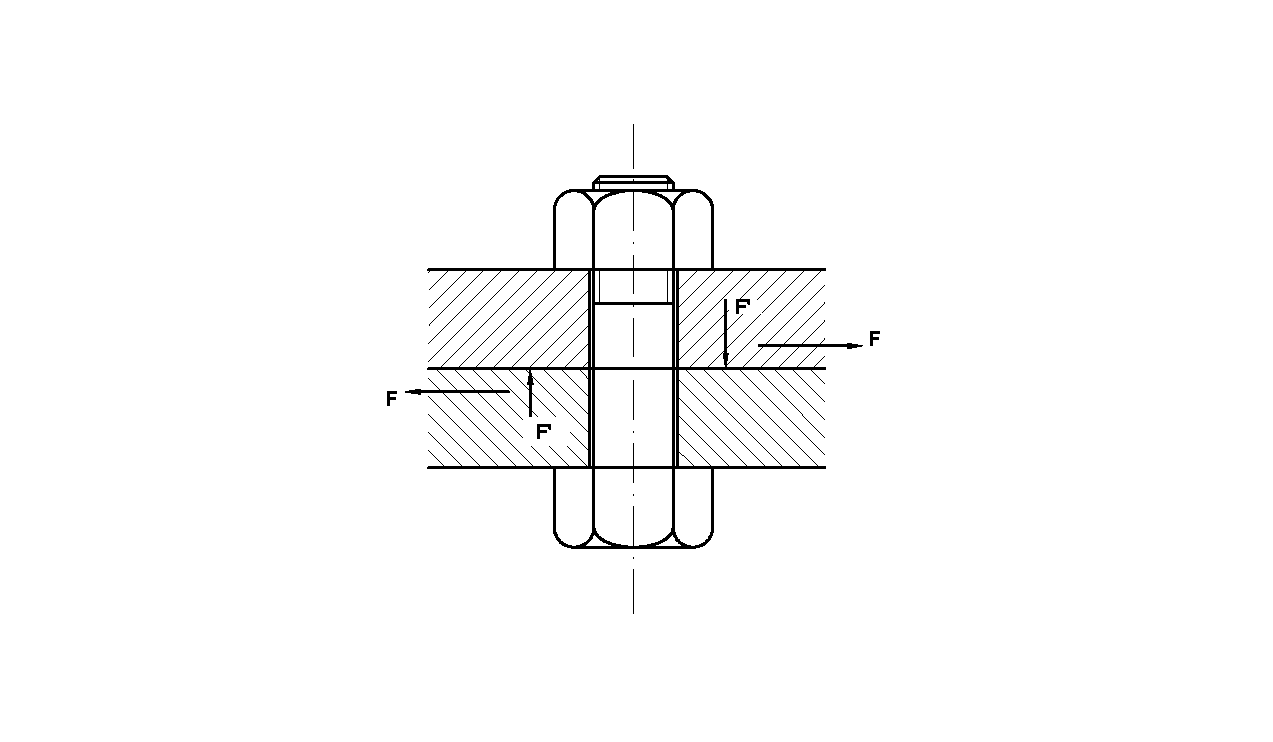
\includegraphics[width=0.9\textwidth]{figures/jiaohe-Model.eps}
	\caption{电池箱安装框架螺栓连接受力模型}\label{fig:jiaohe}
\end{figure}

如图 \ref{fig:jiaohe} 所示的螺栓连接为电池箱底座螺栓连接的模型,在运动的过程中,螺栓仅仅受到剪切力的作用,由于螺栓存在预紧力,所以在连接面产生了摩擦力来抵抗工作载荷,在这种情况下,螺栓体仅仅承受预紧力的作用,而且预紧力的大小并不收到工作载荷的影响。预紧力 $F'$ 的大小计算需要根据在螺栓结合面不产生滑移的条件决定,如式 ,式中的 $F_a$ 为电池箱因为加速度而产生的水平剪切力,$f$ 为接合面的摩擦系数,在这里为 $0.3$,$n$ 为螺栓的数量,为 20,$m$ 为结合面的数量,$m=1$,$Kn$ 为可靠性系数,$Kn=1.1$。经过计算得到的预紧力为 $F'= 413.23 N$

\begin{equation}
	F'=\frac{F_aK_n}{mnf}
\end{equation}

螺栓危险截面需要满足的强度条件如式 \ref{equ:1.3} 所示,经过计算,使用普通碳钢螺栓,材料为 Q235,查表得到其 $R_{eL}=240 \mathrm{MPa}$。选用的螺栓的直径范围为 $d=16~30 mm$,不控制预紧力且工作在变载条件下的安全系数 $S=6.5$。

\begin{equation}
	[\sigma]=\frac{R_{eL}}{[S]}=\frac{240}{6.5}=37 \mathrm{MPa}
\end{equation}

\begin{equation}
	d_1 \geq \sqrt{\frac{5.2F'}{\pi[\sigma]}}=\sqrt{\frac{5.2 \times 413.23}{3.14 \times 37}}=18.4 mm
\end{equation}

由计算得到的电池箱安装框架的螺栓直径应在 $d_1 \geq 18.4 mm $ 以上,故选择的螺栓为 M20 螺栓。

同理,根据以上的计算过程,在电池箱内安装的电池模组的安装螺栓的直径范围为:



\begin{equation}
\begin{aligned}
	F'&=\frac{F_aK_n}{mnf} = 107 N \\
	d_2 &\geq \sqrt{\frac{5.2F'}{\pi[\sigma]}}=\sqrt{\frac{5.2 \times 107}{3.14 \times 37}}=4.79 mm
\end{aligned}
\end{equation}

由此得到的电池箱模组的的螺栓直径应在 $d_2 \geq 4.79 mm $ 以上,故选择的螺栓为 M5 螺栓。

\subsection{垂直方向}

在垂直方向上的校核内容为校核电池箱连接处的材料是否会被预紧力压溃,或者在安装完成后,电池箱底座某位置产生过大的挠度。由于电池箱的内部电池质量较重,故在安装完成的时候,电池箱底板需要承受所有的重量,而一般的电池安装框架只能够在电池箱的四周固定,故电池箱底板的形变和应力状态是电池箱内的危险面 \cite{王兵2014电动汽车电池箱仿真分析及设计优化}。由于电池箱为在三维空间内的物体,故受力状态较为复杂,在本文中利用了 Solidworks 中自带的有限元分析软件来分析电池箱底座的受力变形状态与材料的状态。

在分析受力的时候,将底座连接处固定在夹具上,并向电池箱内部施加压力,用来仿真电池箱在安装完毕的时候,由于内部电池模组对于电池箱安装框架的压力,在计算的时候,力被均匀加载在电池安装框架上。

\subsubsection{应力分析}

在分析应力的时候,采用的应力分析准则为 von Mises 准则,又被称为范式等效应力。该准则综合了各个主应力的作用,被广泛用于材料的应力分析当中,范式等效应力的准则是,当在被分析材料中的某一点所在位置的点应力达到达到某一与应力状态无关的定值时,材料就发生屈服或者压溃现象,换句话说,当材料的弹性势能超过某一界限的时候,就认定材料发生了屈服现象。

对于电池箱安装框架的有限元分析过程,第一步,首先要限定电池箱的机械连接部分,在软件中使用软件提供的夹具功能将电池箱底座与车体相连接的部分固定,在校核的时候,本文认定在机械连接的部分因为已经安装有螺栓,该处已经固定在车体上不因为受到来自电池单体的压力而发生应变;第二步,在电池模组的位置加载等效电池模组对于底座压力的力,因为每个电池单体的质量为 $12 kg$,一共有 8 个模组,重力加速度为 $g=9.8m^2$,在电池箱一共施加的等效力的大小为 $940.8 N$;第三步,为了轻量化设计,电池箱底座的材料选择 1060 铝合金材质,在软件中设置零件的材料为 1060 铝合金。

使用此应力定则分析本文的电池安装框架中可以得到各点处的范式等效应力的大小值,如图 \ref{fig:yingli} 所示,在图中可以看到,材料的范式等效应力范围最大处应力为 5.42 MPa,材料的范式屈服应力值为 27.6 MPa,材料并未发生屈服。

\begin{figure}
	\centering
	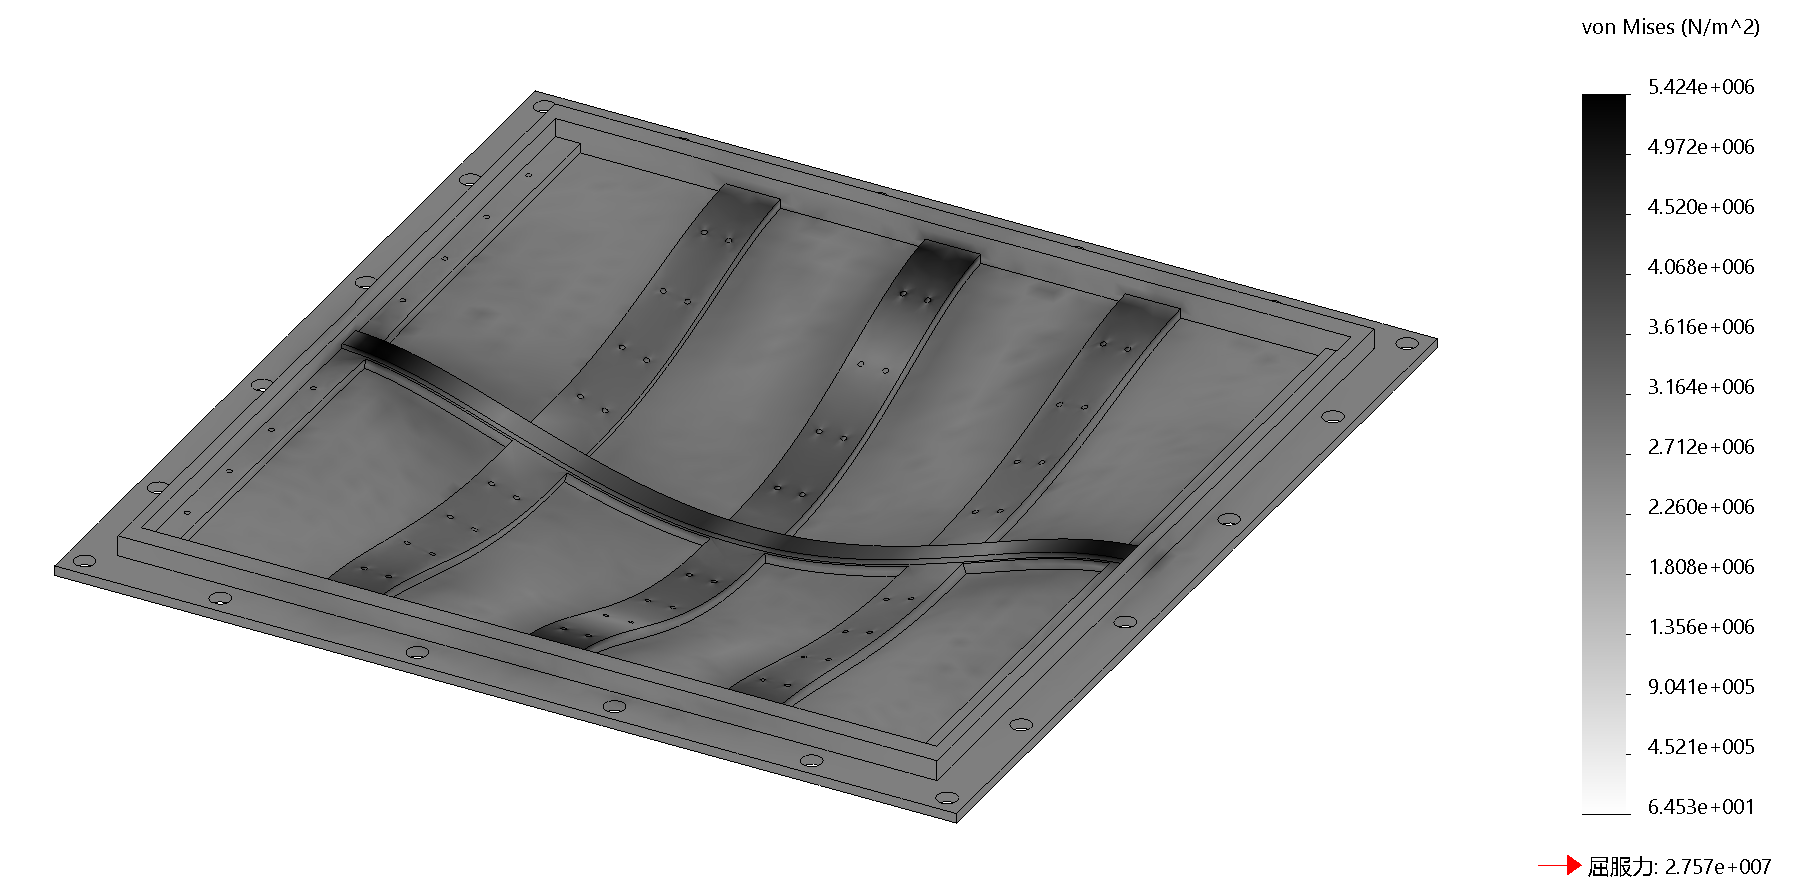
\includegraphics[width=0.9\textwidth]{figures/yingli.png}
	\caption{电池箱安装框架应力分布图(应变放大 500 倍)}\label{fig:yingli}
\end{figure}

根据 Solidworks 提供的应变分析引擎,可以得到电池箱安装框架在安装后的应变分布,如图 \ref{fig:yingbian} 所示,在电池箱底座中,最大应变量为 $0.181 mm$。

\begin{figure}
	\centering
	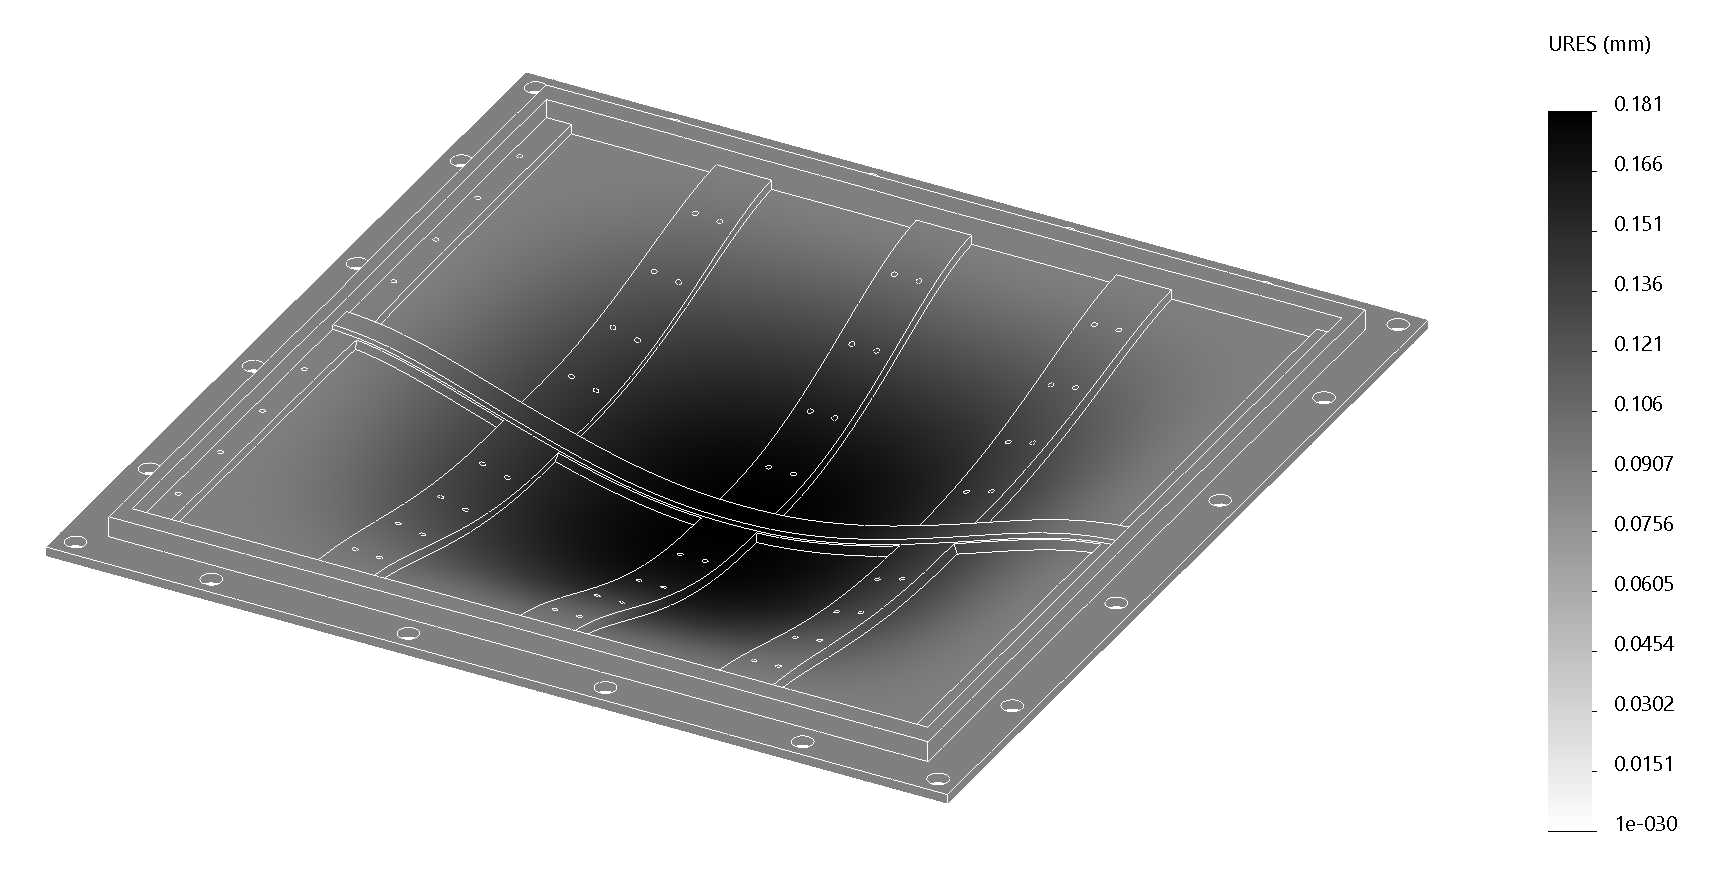
\includegraphics[width=0.9\textwidth]{figures/yingbian.png}
	\caption{电池箱安装框架应变分布图(应变放大 500 倍)}\label{fig:yingbian}
\end{figure}

根据有限元软件校核的结果,可以判断本文设计的电池箱安装框架结构符合使用要求,并且给出了在安装电池模组和在安装电池安装底座的螺栓预紧力的值。